%% DONE
\id{ҒТАМР 06.35.31}{}

\begin{articleheader}
\sectionwithauthors{Д.Х. Беделова, С.Б. Мақыш, А.Б. Алибекова}{МЕМЛЕКЕТТІК АКТИВТЕР ЖӘНЕ ОЛАРДЫ БАСҚАРУДЫҢ ЭКОНОМИКАЛЫҚ МАЗМҰНЫ}

{\bfseries
\textsuperscript{1}Д.Х. Беделова\textsuperscript{\envelope } \authorid,
\textsuperscript{2}С.Б. Мақыш\authorid,
\textsuperscript{1}А.Б. Алибекова\authorid}
\end{articleheader}

\begin{affiliation}
{\em \textsuperscript{1}Л.Н.Гумилев атындағы Еуразия Ұлттық Университеті, Астана, Қазақстан,}

{\em \textsuperscript{2}Esil University, Астана, Қазақстан,}

\textsuperscript{\envelope }Корреспондент-автор: everest-astana@mail.ru
\end{affiliation}

Активтер кәсіпорынның бизнес процесінде пайдаланылатын экономикалық
ресурстардың әртүрлі түрлерін білдіреді. Бұл ресурстар белгілі бір
мақсаттарға жетуге бағытталған ұйымның миссиясы мен экономикалық даму
стратегиясына сәйкес қалыптасады. Өзінің мәні бойынша активтер
кәсіпорынның экономикалық әлеуетінің негізін құрайды, мүліктік
құндылықтар жиынтығы түрінде көрінеді. Экономикалық ресурстардың
мақсатты түрде қалыптасқан тобы ретінде активтер оның стратегиялық
міндеттерін іске асыруды және тұрақты дамуды қамтамасыз ететін
кәсіпорынның шаруашылық қызметінің функционалдық бағыты мен
ерекшеліктеріне сәйкес келуі керек.

Демек, экономикалық сипаттамаларға ие активтер кез келген
микроэкономикалық жүйеде экономиканы басқарудың негізгі объектілеріне
айналады. Олар осы жүйенің тиімді жұмыс істеуі мен тұрақты дамуын
қамтамасыз етуде маңызды рөл атқарады.

Мақалада мемлекет активтерінің экономикалық мәні, мазмұны және оларды
басқару тәсілдері қарастырылады. Мақаланың маңыздылығы -- экономикалық
тұрақтылық пен дамудың негізі ретіндегі мемлекеттік активтердің
маңыздылығы туралы терең түсінік беру. Мемлекеттік активтерді басқарудың
әртүрлі аспектілерін талдай отырып, мақалада олардың тиімділігі мен
тұрақтылығын арттыру бойынша ұсыныстар берілген. Мұның экономикалық
саясатты қалыптастыруға және жүзеге асыруға жауапты мемлекеттік органдар
үшін, сондай-ақ экономикалық ресурстарды басқару мәселелерін зерттейтін
ғалымдар мен практиктер үшін тікелей практикалық маңызы бар.

{\bfseries Түйін сөздер:} активтер,қаржылық активтер, мүлік, мемлекеттік
активтер, мемлекеттік басқару, мемлекеттік қаражаттар

\begin{articleheader}
{\bfseries ГОСУДАРСТВЕННЫЕ АКТИВЫ И ЭКОНОМИЧЕСКОЕ СОДЕРЖАНИЕ УПРАВЛЕНИЯ ИМИ}

{\bfseries
\textsuperscript{1}Д.Х. Беделова\textsuperscript{\envelope },
\textsuperscript{2}С.Б. Мақыш,
\textsuperscript{1}А.Б. Алибекова}
\end{articleheader}

\begin{affiliation}
{\em \textsuperscript{1}Евразийский Национальный Университет имени Л.Н.Гумилев, Астана, Казахстан,}

{\em \textsuperscript{2} EsilUniversity, г.Астана, Казахстан,}

\emph{e-mail: everest-astana@mail.ru}
\end{affiliation}

Активы представляют собой различные виды экономических ресурсов,
используемых в бизнес-процессе предприятия. Эти ресурсы формируются
согласно миссии организации и стратегии экономического развития,
направленной на достижение определенных целей. По своей сути активы
составляют основу экономического потенциала предприятия и выступают в
виде совокупности имущественных ценностей. Как целенаправленно
сформированная группа экономических ресурсов активы должны
соответствовать функциональному направлению и особенностям экономической
деятельности предприятия, что обеспечивает реализацию его стратегических
целей и устойчивое развитие.

Поэтому активы, обладающие экономическими характеристиками, становятся
основными объектами экономического управления в любой микроэкономической
системе. Они играют важную роль в обеспечении эффективного
функционирования и устойчивого развития этой системы. В статье
рассматривается экономическое значение, содержание и способы управления
государственными активами. Важность статьи заключается в том, чтобы дать
более глубокое понимание значения государственных активов как основы
экономической стабильности и развития. Анализируя различные аспекты
управления государственными активами, в статье даются рекомендации по
повышению их эффективности и устойчивости. Это имеет прямое практическое
значение для государственных органов, ответственных за формирование и
реализацию экономической политики, а также для ученых и практиков,
изучающих вопросы управления экономическими ресурсами.

{\bfseries Ключевые слова:} активы, финансовые активы, имущество,
государственные активы, государственное управление, государственные
фонды.

\begin{articleheader}
{\bfseries STATE ASSETS AND THE ECONOMIC CONTENT OF THEIR MANAGEMENT}

{\bfseries
\textsuperscript{1}D.H. Bedelova\textsuperscript{\envelope },
\textsuperscript{2}S.B. Makysh,
\textsuperscript{1}A.B. Alibekova}
\end{articleheader}

\begin{affiliation}
{\em \textsuperscript{1}L.N.Gumilyov Eurasian National University, Astana, Kazakhstan,}

{\em \textsuperscript{2}Esil University, Astana, Kazakhstan,}

\emph{e-mail: everest-astana@mail.ru}
\end{affiliation}

Assets are various types of economic resources used in the business
process of an enterprise. These resources are formed according to the
mission of the organization and the strategy of economic development
aimed at achieving certain goals. In essence, assets form the basis of
the economic potential of an enterprise and act as a set of property
values. As a purposefully formed group of economic resources, assets
must correspond to the functional direction and features of the economic
activity of the enterprise, which ensures the implementation of its
strategic goals and sustainable development. Therefore, assets with
economic characteristics become the main objects of economic management
in any microeconomic system. They play an important role in ensuring the
effective functioning and sustainable development of this system. The
article considers the economic significance, content and methods of
managing state assets. The importance of the article lies in giving a
deeper understanding of the significance of state assets as the basis
for economic stability and development. Analyzing various aspects of
state asset management, the article provides recommendations for
increasing their efficiency and sustainability. This is of direct
practical importance for government agencies responsible for the
formation and implementation of economic policy, as well as for
scientists and practitioners studying the management of economic
resources.

{\bfseries Keywords:} assets, financial assets, property, state assets,
public administration, public funds.

\begin{multicols}{2}
{\bfseries Кіріспе.} Мемлекеттік активтерді экономикалық қамтамасыз ету
және басқару ұлттық экономиканың қызмет етуінің орталық элементі болып
табылады. Мемлекеттік активтерге жер, ғимараттар, инфрақұрылым, табиғи
ресурстар және мемлекеттік кәсіпорындар сияқты әртүрлі ресурстар кіреді.
Бұл активтерді тиімді басқару тұрақты экономикалық өсімге қол жеткізу,
халықтың әл-ауқатын арттыру және азаматтардың өмір сүру сапасын жақсарту
үшін маңызды. Бұл басқару ресурстарды пайдалануды оңтайландыруды, оларды
жаңғыртуды және ұтымды бөлуді қамтиды, бұл экономикалық тұрақтылықты
нығайтуға және мемлекеттің дамуына ықпал етеді.

Жаһандану, өзгермелі экономикалық жағдайлар мен жылдам технологиялық
прогресстен туындайтын заманауи сын-қатерлер мемлекеттік активтерді
басқарудың дәстүрлі тәсілдерін түбегейлі қайта қарауды талап етеді.
Негізгі міндет -- ұлттық байлықты сақтап, көбейту ғана емес, оны
еліміздің стратегиялық даму мақсаттарына жету үшін ұтымды пайдалану. Бұл
мақалада мемлекеттік активтерді басқарудың терең теориялық және
практикалық аспектілері қарастырылады. Оларды бағалау және оңтайландыру
үшін қолданылатын заманауи әдістер мен құралдарға жан-жақты талдау
жүргізіледі. Мемлекеттік ресурстарды пайдалану тиімділігін арттыруға
бағытталған жекешелендіру, мемлекеттік-жекешелік әріптестік және
инвестициялық саясат мәселелеріне ерекше назар аударылады. Бұл
аспектілер олардың тұрақты экономикалық өсуді қамтамасыз етудегі және
әлеуметтік әл-ауқатты жақсартудағы рөлі контекстінде қарастырылады.

Бұл зерттеудің мақсаты -- мемлекеттік активтерді басқару жүйесін олардың
мемлекеттік басқаруда практикалық қолдану мүмкіндігіне баса назар аудара
отырып, кешенді талдау. Зерттеу жетістіктің негізгі факторлары мен
реформалардың әлеуетті бағыттарын анықтау үшін халықаралық тәжірибе мен
озық тәжірибеге сүйенеді.

Зерттеудің өзектілігі мемлекеттік басқару тәжірибесін жаңа экономикалық
жағдайларға бейімдеу қажеттілігімен және мемлекеттік ресурстарды
пайдаланудағы ашықтық пен тиімділік стандарттарының жоғарылауымен
байланысты. Ол мемлекеттік активтерді басқаруды оңтайландыру арқылы
елдің экономикалық тұрақтылығы мен дамуын жақсарту үшін ғылыми
негізделген шешімдер мен нақты ұсыныстар әзірлеуге бағытталған.

Зерттеудің гипотезасы. Заманауи басқару әдістері мен экономикалық
бағалауды қолдану негізінде мемлекеттік активтерді тиімді басқару
олардың құнын арттыруға, ұтымды пайдалануға және экономиканың тұрақты
дамуына ықпал етеді. Бақылау, талдау және есепке алу тетіктерін
жетілдіру арқылы мемлекет активтерін басқаруды оңтайландыру олардың
мемлекет мүддесі үшін тиімдірек пайдаланылуын қамтамасыз етеді,
экономикалық өсуге және қоғамның әл-ауқатын арттыруға ықпал етеді.

Мемлекеттік активтерді басқаруды жетілдіру бойынша ұсыныстарды зерттеу
және енгізу шығындарды азайтуға, активтердің табыстылығын арттыруға және
оларды пайдалануды оңтайландыруға мүмкіндік береді деп күтілуде. Бұл
мемлекеттік ресурстарды неғұрлым ұтымды бөлуді және оларды пайдаланудың
жалпы экономикалық тиімділігін арттыруды қамтамасыз етеді.

{\bfseries Материалдар мен әдістер.} Экономикалық қауіпсіздік пен
мемлекеттік активтерді тиімді басқару ұлттық экономиканың тұрақты
дамуының негізі болып табылады. Мемлекеттік активтер материалдық
ресурстарды ғана емес, сонымен бірге елдің әлеуметтік-экономикалық
құрылымының негізін, оның ішінде жерді, ғимараттарды, инфрақұрылымды,
табиғи ресурстарды және кәсіпорындарды білдіреді. Бұл активтерді тиімді
басқару экономикалық өсу үшін қолайлы жағдайлар жасау, азаматтардың өмір
сүру деңгейін жақсарту және ұзақ мерзімді тұрақтылықты қамтамасыз ету
үшін өте маңызды.

Бұл мақалада мемлекеттік активтерді басқарудың теориялық және
практикалық аспектілерінің терең талдауы, оның ішінде осы активтерді
бағалау мен оңтайландырудың заманауи әдістері мен құралдарын
егжей-тегжейлі зерделеу қарастырылған. Жекешелендіру,
мемлекеттік-жекеменшік әріптестікті дамыту және мемлекеттік ресурстарды
пайдалану тиімділігін арттыруға бағытталған инвестициялық саясатты
қалыптастыру мәселелеріне ерекше назар аударылады.

Осы зерттеу үшін келесі әдістер қолданылды: статистика саласындағы
уәкілетті мемлекеттік органмен ұсынылған мәліметтерді талдау, салыстыру,
зерттеу мемлекет активтерінің динамикасын зерттеуге мүмкіндік берді.

Қорытындыларды негіздеу үшін мақалада эмпирикалық зерттеу әдістері
қолданылады. Бақылау, оның ішінде қаржылық есеп беру және статистика
арқылы мемлекеттік активтерінің ағымдағы жағдайын талдау қолданылды.

Қазіргі жағдайларда мемлекеттік басқару тәжірибесін тез өзгеретін
экономикалық шындыққа және ашықтық пен басқару тиімділігіне қойылатын
талаптардың артуына бейімдеу ерекше маңызды. «Актив» термині қаржылық
құралдарды, инфрақұрылымды, ғимараттарды, жабдықтарды, негізгі
құралдарды, машиналарды және экономикалық құндылығы бар және табыс
немесе пайда әкелуге қабілетті басқа да материалдық активтерді қамтуы
мүмкін мүлік пен ресурстардың алуан түрлерін сипаттау үшін қолданылады
{[}1{]}. Осылайша, активтерді басқару ресурстарды тиімді басқаруды ғана
емес, сонымен қатар ұйымның экономикалық өнімділігін және бәсекеге
қабілеттілігін қамтамасыз етудегі олардың рөлін терең түсінуді талап
етеді.

\emph{Әдебиетке шолу}{\bfseries .} Активтер күрделі салымдар арқылы
жасалған жинақталған мүліктік құндылықтарды білдіреді. Бұл капиталды
жаңа бизнесті құрудың басында да, ұйымдық активтерді қалыптастыра
отырып, оның кейінгі дамуына да салуға болады. Капитал мен активтер
арасындағы байланыс қарапайым қаржылық байланысқа қарағанда тереңірек:
активтер инвестицияны жай ғана қабылдап қоймайды, олар экономикалық
қызмет барысында табыс пен пайда түрінде капиталды қайтарудың негізіне
айналады. Капитал мұнда тек қаржылық ресурс ретінде ғана емес, сонымен
қатар өндіріс орындары мен технологиялар сияқты нақты активтерге
инвестициялау арқылы ұйымды нығайту мен өсіруге бағытталған стратегиялық
құрал ретінде де әрекет етеді.

Активтер -- ұйымның экономикалық мәніне қарай бағаланатын құнды мүліктік
ресурстары. Олардың құнын анықтау жасау шығындары, пайдалану ұзақтығы,
бизнес мақсаттары және нарықтық жағдайлар сияқты бірқатар факторларды
қамтиды. Бұл аспектілер активтің жалпы құнын қосады {[}2{]}. Әртүрлі
зерттеушілер мен ғалымдар ұсынған активтер түсінігін терең түсіну үшін
сөздік анықтамалары көбінесе активтердің мәнін жеңілдететінін, олардың
жасалу мақсаттарына, қоғамда міндетті түрде пайдаланылуына әрдайым назар
аудармайтынын ескеру қажет. кәсіпорынның шаруашылық қызметі, сондай-ақ
олардың қаржылық есеп берудегі көрінісі.

«Активтер» ұғымына қатысты әртүрлі көздерден алынған анықтамалар
1-кестеде көрсетілген.
\end{multicols}

\begin{table}[H]
\caption*{1 - кесте. Активтер» ұғымына қатысты әртүрлі көздерден алынған анықтамалар}
\centering
\begin{tblr}{
  colspec = {X[2] X[5]},
  row{1} = {c},
  cell{7}{1} = {c=2}{},
  hlines,
  vlines,
}
Дереккөз                                                                                                            & Определение активов                                                                                                                                                                                                                                  \\
Андросов, А. М.                                                                                                     & «Материалдық, қаржылық және материалдық емес активтерден тұратын мүлік» [3].                                                                                                                                                                         \\
Акатьева, М. Д.,Бирюков, В. А.                                                                                      & «Жеке немесе заңды тұлғаға тиесілі мүліктік, мүліктік және мүліктік емес құқықтардың (мүліктік) жиынтығы» [4].                                                                                                                                       \\
Экономикалық-математикалық сөздік                                                                                   & «Активтер табыс (пайда) немесе басқа да пайда әкелуге қабілеті» [5].                                                                                                                                                                                 \\
Р.М. Нуриев                                                                                                         & «Өз иесіне тікелей төлемдер (пайда, дивидендтер, рента және т.б.) түрінде де, кәсіпорынның, жылжымайтын мүліктің, акциялардың және т.б. құнын арттыру үшін жасырын төлемдер түрінде де ақша қаражаттарының қозғалысын қамтамасыз ететін қорлар» [6]. \\
«Бухгалтерлік есеп және қаржылық есептілік туралы» Қазақстан Республикасының 2007 жылғы 28 ақпандағы № 234-III Заңы & Активтер – болашақ экономикалық пайдалар күтілетін өткен оқиғалардың нәтижесінде жеке тұлға немесе ұйым бақылайтын ресурстар.                                                                                                                        \\
Ескерту: дереккөздер негізінде авторлармен құрастырылған                                                            &                                                                                                                                                                                                                                                      
\end{tblr}
\end{table}

\begin{multicols}{2}
Р.М.Нуриев өз анықтамасында активтерден туындайтын ақша ағындарының
маңыздылығын атап көрсетеді, бірақ осы категорияға енуі мүмкін
ресурстардың нақты түрлерін көрсетпейді және осы активтердің
ерекшеліктерін немесе бірегей сипаттамаларын ашпайды {[}6{]}. Е.С.
Денисенко мен Ю.Н. Воробьев активтерге ұқсас және барынша толық
анықтамалар береді {[}7{]}.

Активтер ұйымның қаржылық жағдайын нығайтуға көмектесетін қарыздық
міндеттемелерді өтеу үшін төлем құралы ретінде қызмет ете алады.
«Активтер» түсінігін тереңірек түсіну үшін Халықаралық қаржылық
есептілік стандарттарына және Мемлекеттік секторға арналған халықаралық
қаржылық есептілік стандарттарына (ХҚЕС) сілтеме жасау ұсынылады, мұнда
бұл тұжырымдама қаржылық есептілік контекстінде жүйеленген және ашылған.
Біздің түсінігіміз бойынша активтер ұйымның шаруашылық қызметін жүзеге
асыру процесінде қолданылатын әртүрлі экономикалық ресурстарды
білдіреді. Соңғы жылдары Қазақстанда мемлекет меншік құқығын нығайту
және жеке сектормен қарым-қатынасын реформалау бойынша белсенді жұмыс
жүргізуде. Бұл әсіресе мұнай, газ, кен сияқты пайдалы қазбаларды өндіру
арқылы ел экономикасында шешуші рөл атқаратын шикізат секторында
байқалады. Бұл күш-жігер жалпы экономиканың дамуына ықпал ете отырып,
ұлттық ресурстарды пайдаланудың басқару мен экономикалық тиімділігін
арттыруға бағытталған. Бүгінгі таңда Қазақстандағы ұлттық компаниялар
өздерінің заңды өкілеттіктерін нақтылау және кеңейту қажеттілігімен
бетпе-бет келіп отыр. Негізінен мұнай-газ секторының нақты талаптарына
бағытталған негізгі заңнамалық база ұлттық компаниялардың экономиканың
басқа салаларындағы мүмкіндіктерін шектейді. Ұлттық компаниялардың
өкілеттіктерін және олардың ұйымдастырушылық өзгерістерін нақтылау үшін
нормативтік актілер үнемі жаңартылып отырады. Сондай-ақ экономика
салаларының стратегиялық дамуындағы ұлттық компаниялардың рөлі мен
функцияларын анықтауға және олардың индустриялық дамудың негізгі
мәселелерін шешуге ықпалын шектеуге басты назар аударылады. Терең талдау
негізінде біз активтерді жіктеуге келесі тәсілді ұсынамыз (1-сурет).
\end{multicols}

\begin{figure}[H]
	\centering
	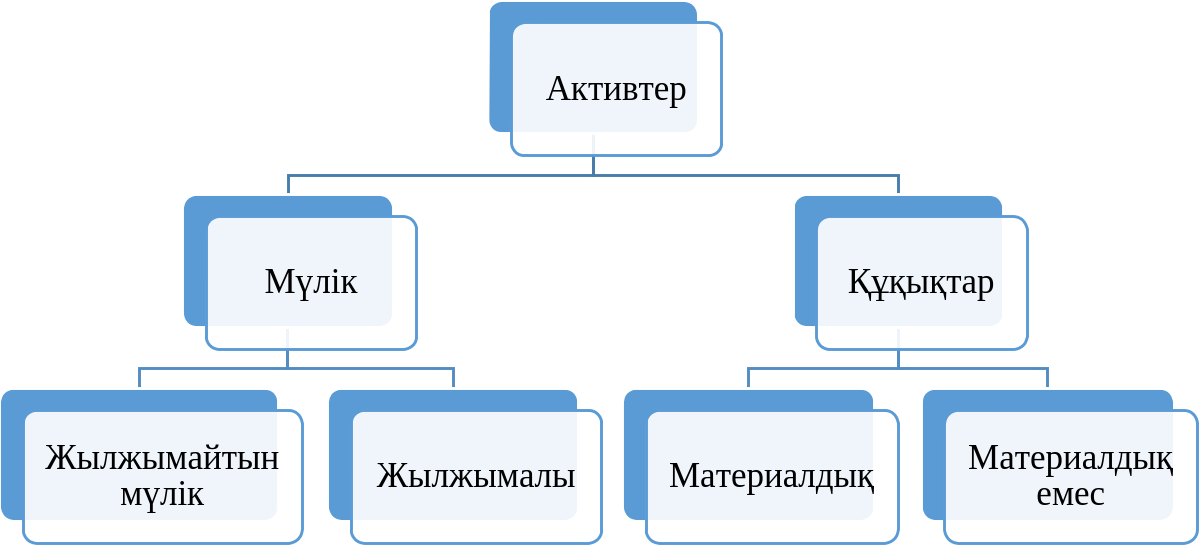
\includegraphics[width=0.75\textwidth]{media/ekon2/image11}
	\caption*{1 - сурет. Активтердің түрлері бойынша жіктелуі}
	\caption*{Ескертпе - Дереккөздер негізінде құрастырған автор {[}8{]}}
\end{figure}

\begin{multicols}{2}
Мемлекеттiк активтер -- бұл мемлекеттiк субъектiнiң толық бақылауындағы
экономикалық ресурстар. Бұл бақылау ұйымның пайдаланылған экономикалық
ресурстарға немесе белгілі бір жағдайларда заңға сәйкес меншік құқығына
ие болуын білдіреді, мысалы, қаржылық лизингті пайдалану кезінде.

Мемлекеттік органдар әлеуметтік-экономикалық мақсаттарға жету және өз
функцияларын орындау үшін әртүрлі мемлекеттік қаржылық және басқа
ресурстарды пайдаланады. Бұл ресурстар әдебиетте қоғамдық қорлар немесе
қауымдастық ресурстары ретінде де сипатталады. Мемлекет активтерінің
құрылымы мен құрамы әртүрлі ғылыми-практикалық зерттеулерде жан-жақты
зерттеледі. Мемлекеттiк активтерге мемлекет өз мақсаттарына жету және өз
функцияларын орындау үшiн пайдаланатын әр түрлi ресурстар жатады. Бұл
активтерді бірнеше негізгі санаттарға бөлуге болады. Бірінші санатқа
алтын-валюта резервтері, мемлекеттік бағалы қағаздар және әртүрлі
қаржылық механизмдер, соның ішінде салық және кедендік құралдар сияқты
физикалық және қаржылық активтер кіреді. Бұған әртүрлі деңгейдегі
бюджеттік жүйелерді біріктіретін мемлекеттік қорлар да кіреді. Екінші
категорияға шаруашылық жүргізуші субъектілер мен басқа шаруашылық
жүргізуші субъектілердің меншігіндегі әртүрлі меншік нысандарын
білдіретін экономикалық қорлар жатады.

Мемлекеттік активтерді басқаруда мемлекет қаражатын пайдалану
тиімділігін бағалау мемлекеттік аудиттегі ең күрделі міндеттердің бірі
болып табылады. Әлеуметтік дамуды бақылауда әлеуметтік көрсеткіштер
сияқты сандық көрсеткіштер шешуші рөл атқарады. Олар қоғамның қазіргі
жағдайын бағалауға ғана емес, сонымен бірге оның қайта құруларын
қадағалауға, тенденцияларды, дағдарыс құбылыстарын анықтауға және
қабылданған басқару шешімдерінің сапасын бағалауға мүмкіндік береді.

Мемлекеттік аудит бұл ақпаратты жинау мен талдауда, оны қоғамдық
пайдалану үшін қолжетімді етуде және үкіметтің жауапкершілігін күшейтуде
маңызды рөл атқарады. Сыртқы мемлекеттік аудит және қаржылық бақылау
органдарының сараптамалық-талдау қызметін жүргізуін реттейтін 903
процедуралық стандарттың маңызы ерекше ға ие. Осы стандарт тексерілетін
ұйымдардың жағдайын бағалауға, дағдарыстық жағдайлардың себептерін
анықтауға және мемлекеттік органдар мен кәсіпорындардың жұмысына әсер
ететін факторларды талдауға бағытталған әртүрлі аналитикалық
процедураларды қолдануды қарастырады.

{\bfseries Нәтижелер мен талқылау.} Мемлекет активтерінің бұл құрамдас
бөліктері мемлекеттің экономикалық және әлеуметтік саясатында негізгі
рөл атқарады, экономикалық ресурстарды тұрақты басқаруды және
стратегиялық даму мақсаттарын жүзеге асыруды қамтамасыз етеді.
Мемлекеттік активтерге мемлекеттің функцияларын орындауға және оның
стратегиялық мақсаттарына қол жеткізуге қажетті әртүрлі ресурстар
жатады. Бұл активтерді бірнеше негізгі санаттарға бөлуге болады.
Мемлекеттiк активтердiң осы түрлi құрамдас бөлiктерi экономиканы
басқаруда және ұлттық қауiпсiздiктi қамтамасыз етуде маңызды рөл
атқарады, тұрақты дамуға және мемлекеттiң әлеуметтiк-экономикалық
мақсаттарына қол жеткiзуге ықпал етедi.
\end{multicols}

\begin{figure}[H]
	\centering
	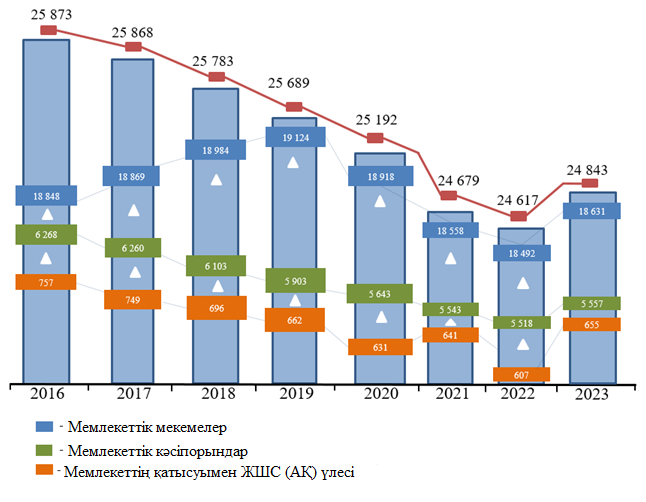
\includegraphics[width=0.8\textwidth]{media/ekon2/image2}
	\caption*{2 - сурет. Мемлекет қатысатын ұйымдар санының динамикасы}
	\caption*{Ескертпе - Дереккөздер негізінде құрастырған автор {[}9{]}}
\end{figure}

\begin{multicols}{2}
Ұйым пайдаланатын, бірақ бақыламайтын мемлекеттік активтерді оның жеке
активтері ретінде тануға болмайды. Бұл, ең алдымен, еңбек ресурстарына,
сондай-ақ ұйым уақытша тегін пайдалануға жалға алатын немесе алатын
мүлікке қатысты. Өз кезегінде, мемлекеттік актив деп мемлекеттік
қатысатын ұйымдар жатады. Мемлекет қатысатын ұйымдар санының динамикасы
2 суретте көрсетілген.

Ұйымдастырушылық-құқықтық нысандары бойынша: мемлекеттік мекемелер -
18631, қазыналық кәсіпорындар - 5557, мемлекет қатысатын АҚ (ЖШС) (шетел
қатысуынсыз) - 655 (2-кесте).
\end{multicols}

\begin{table}[H]
\caption*{2 - кесте. Мемлекет қатысатын ұйымдар санының динамикасы, бірлік}
\centering
\begin{tblr}{
  colspec = {X[2] X[1] X[1] X[1]},
  row{2} = {c},
  cell{1}{1} = {r=2}{},
  cell{1}{2} = {c=3}{c},
  cell{3}{2} = {c},
  cell{3}{3} = {c},
  cell{3}{4} = {c},
  cell{4}{2} = {c},
  cell{4}{3} = {c},
  cell{4}{4} = {c},
  cell{5}{2} = {c},
  cell{5}{3} = {c},
  cell{5}{4} = {c},
  cell{6}{2} = {c},
  cell{6}{3} = {c},
  cell{6}{4} = {c},
  cell{7}{2} = {c},
  cell{7}{3} = {c},
  cell{7}{4} = {c},
  cell{8}{2} = {c},
  cell{8}{3} = {c},
  cell{8}{4} = {c},
  cell{9}{2} = {c},
  cell{9}{3} = {c},
  cell{9}{4} = {c},
  cell{10}{2} = {c},
  cell{10}{3} = {c},
  cell{10}{4} = {c},
  cell{11}{2} = {c},
  cell{11}{3} = {c},
  cell{11}{4} = {c},
  cell{12}{1} = {c=4}{},
  vlines,
  hline{1,3-13} = {-}{},
  hline{2} = {2-4}{},
}
Ұйымдастырушылық-құқықтық нысаны                                   & Мемлекеттік меншік                     &                                        &            \\
                                                                   & 2022 жылғы 1 қаңтардағы жағдай бойынша & 2023 жылғы 1 қаңтардағы жағдай бойынша & Ауытқу, \% \\
Мемлекеттік мекемелер, барлығы                                     & 18 492                                 & 18 631                                 & 0,75       \\
оның ішінде:                                                       &                                        &                                        &            \\
республикалық                                                      & 2 595                                  & 2 763                                  & 6,47       \\
коммуналдық                                                        & 15 897                                 & 15 868                                 & -0,18      \\
Мемлекеттік кәсіпорындар, барлығы                                  & 5 518                                  & 5 557                                  & 0,71       \\
республикалық                                                      & 204                                    & 210                                    & 2,94       \\
коммуналдық                                                        & 5 314                                  & 5 347                                  & 0,62       \\
АҚ (ЖШС) мемлекеттің қатысуымен (шетелдік тұлғалардың қатысуынсыз) & 607                                    & 655                                    & 7,91       \\
БАРЛЫҒЫ:                                                           & 24 617                                 & 24 843                                 & 0,92       \\
Ескерту: дереккөздер негізінде авторлармен құрастырылған [9]       &                                        &                                        &            
\end{tblr}
\end{table}

\begin{table}[H]
\caption*{3 - кесте. Мемлекеттік меншіктен түсетін кірістер, млн теңге}
\centering
\begin{tblr}{
  colspec = {X[2] X[1] X[1] X[1]},
  column{even} = {c},
  column{3} = {c},
  cell{5}{1} = {c=4}{},
  hlines,
  vlines,
}
Көрсеткіштер                                                               & 2020 ж.  & 2021 ж. & 2022 ж. \\
Мемлекеттік кәсіпорындардың таза табысының бір бөлігін алу                 & 2525,4   & 3 952,0 & 4 640,2 \\
Мемлекетке тиесілі акциялардың мемлекеттік пакеттері бойынша дивидендтер   & 138875,1 & 140827  & 116350  \\
Мемлекет меншігіндегі заңды тұлғаларға қатысу үлестерінен түсетін кірістер & 4489,0   & 4696    & 4871    \\
Ескерту: дереккөздер негізінде авторлармен құрастырылған [9]               &          &         &         
\end{tblr}
\end{table}

\begin{multicols}{2}
2021 жылмен салыстырғанда есепті жылы мемлекет қатысатын ұйымдар саны
226-ға өсті, оның ішінде: мемлекеттік мекемелер - 139, мемлекеттік
кәсіпорындар - 39 және мемлекеттің қатысуымен (шетел қатысуынсыз) АҚ
(ЖШС) - 48. Мемлекеттік меншіктен түсетін кірістер 3 кестеде
көрсетілген.

Мемлекеттік кәсіпорындардың таза пайдасынан түскен кіріс 2020 жылы
2525,4 млн теңгеден 2022 жылы 4640,2 млн теңгеге дейін өсті, оң динамика
көрсетті. Заңды тұлғалардағы қатысу үлестерінен түскен кірістер де 4 489
миллион теңгеден 4 871 миллион теңгеге дейін өсті. Алайда, мемлекеттік
акциялар бойынша дивидендтер 2021 жылы 140 827 миллион теңгеден 2022
жылы 116 350 миллион теңгеге дейін (-17,4\%) азайып, жалпы кірістің 2021
жылғы 149 475 миллион теңгеден 125 862 миллион теңгеге дейін (125 862
миллион теңгеге) төмендеуіне әкелді15. Бұл дивидендтік саясатты және
акционерлік активтерді басқаруды оңтайландыру қажеттілігін көрсетеді.
Активтердің табыстылығын, пайдалануын және тозуын үздіксіз талдау
проблемалық аймақтарды анықтауға және олардың өнімділігін арттыру
шараларын қабылдауға мүмкіндік береді.

Демек, ұйымның билігіндегі мүлік мемлекет меншігінде қалады. Бұл
мүліктер республикалық, коммуналдық және басқалар сияқты мемлекеттік
меншіктің әртүрлі нысандарында болуы мүмкін. Нәтижесінде ұйым осы
активтердің иесі емес, уақытша пайдаланушы немесе басқарушы ретінде
әрекет етеді. Ұйымның мүлкіне қаржыландыру көздеріне қарамастан оның
бүкіл мүлкі кіреді. Бұл өз қаражаты да, несие арқылы алынған ресурстар
да, солардың көмегімен сатып алынған мүлік те болуы мүмкін.
Республикалық мүлікке мемлекеттік қазына, сондай-ақ Қазақстан
Республикасы Азаматтық кодексінің 192-бабының 2-тармағының 1-бөлігінде
көрсетілгендей, заңнамалық актілерге сәйкес мемлекеттік республикалық
заңды тұлғаларға бекітілген мүлік жатады. Мемлекеттік активтерді түрлері
бойынша жіктелуі 3 суретте көрсетілген.
\end{multicols}

\begin{figure}[H]
	\centering
	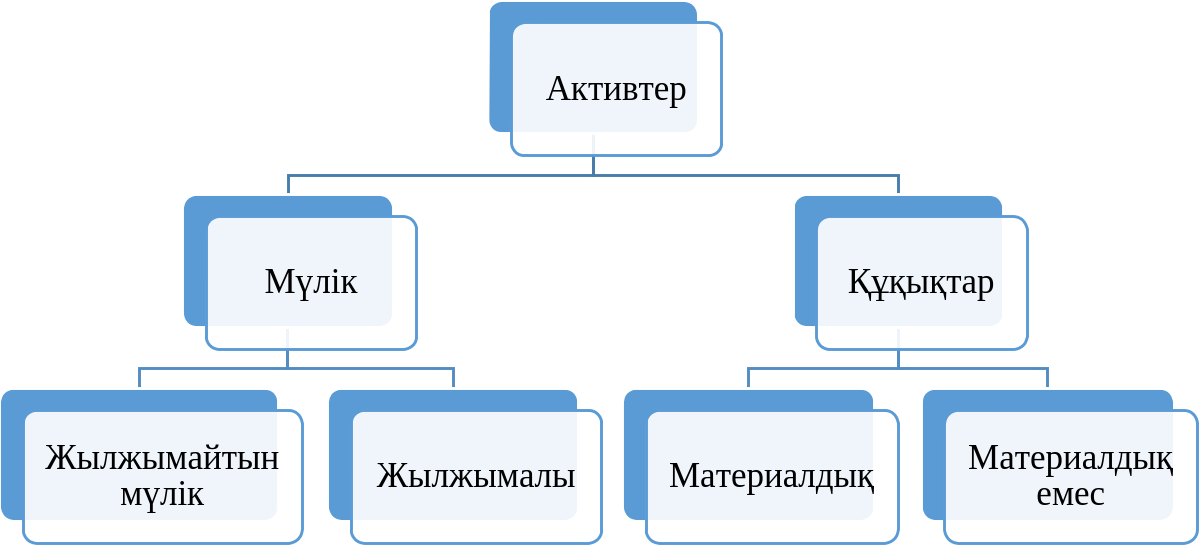
\includegraphics[width=0.7\textwidth]{media/ekon2/image11}
	\caption*{3 - сурет. Мемлекеттік активтерді түрлері бойынша жіктелуі}
	\caption*{Ескертпе - Дереккөздер негізінде құрастырған автор {[}10-11{]}}
\end{figure}

\begin{multicols}{2}
Осылайша, мемлекеттік республикалық заңды тұлғаларға бекітіліп
берілмеген кез келген мүлік Қазақстан Республикасының мемлекеттік
қазынасын құрайды.

Коммуналдық меншікке жергілікті қазына мен заңға сәйкес коммуналдық
заңды тұлғаларға берілген мүлік жатады. Жергілікті бюджет қаражаты және
мемлекеттік заңды тұлғаларға бекітіліп берілмеген өзге де коммуналдық
мүлік Қазақстан Республикасы Азаматтық кодексінің 192-бабының
3-тармағында көрсетілгендей жергілікті қазынаны құрайды. Коммуналдық
меншік жергілікті мемлекеттік басқару деңгейіне қарай облыстық
(республикалық маңызы бар қалалар мен астана үшін) және аудандық
(облыстық маңызы бар қалалар үшін) болып жіктеледі {[}12{]}.

Сонымен бірге, мемлекеттік активтер материалдық (жылжымайтын мүлік,
инфрақұрылым), материалдық емес (зияткерлік меншік), табиғи ресурстар
(мұнай, газ, ормандар) және қаржылық (қорлар, қорлар) болып жіктеледі.

Мемлекеттік активтер -- бұл табыс әкеліп қана қоймай, сонымен бірге
экономикалық дамуға әсер ететін экономикалық ресурстар. Бұл активтерді
басқаруда операциялық немесе инвестициялық қызмет арқылы кіріс алу
мүмкіндігі маңызды рөл атқарады. Олар әлеуетті кіріс көздері ғана емес,
экономиканың белсенді өндірістік элементтері болып табылады. Дегенмен,
олардың табыс алу қабілеті толығымен олардың қаншалықты тиімді
пайдаланылғанына және басқарылатынына байланысты.

Экономикалық қызметке тартылған мемлекеттік активтер үнемі айналымда
болады, бұл осы активтердің барлық түрлеріне және олардың кешеніне
ортақ.

Айналым процесі кезінде активтер түрленеді -- мысалы,
тауарлы-материалдық қорлар дайын өнімге, кейіннен дебиторлық берешекке
немесе ақша қаражатына айналуы мүмкін. Бұл динамикалық процесс
активтердің әртүрлі нысандары арасындағы күрделі өзара әрекеттесулер мен
ауысуларды қамтиды, олардың экономикалық жүйедегі өзгермелілігі мен
жан-жақтылығын көрсетеді.

Жұмыс күшінің және басқа ресурстардың құнының өсуіне байланысты дайын
өнім қорлары сияқты мемлекеттік активтер құнының өзгеруі айналыс
процесінде жиі кездесетін құбылыс болып табылады. Сонымен қатар, негізгі
құралдар мен амортизацияланатын материалдық емес активтер сияқты басқа
активтердің құны тозуға немесе ескіруге байланысты төмендеуі мүмкін.

Мемлекет активтерінің айналымы үш негізгі кезеңді қамтиды: экономикалық,
өндірістік процестерде активтер пайдаланылған кезде; операциялық, олар
белсенді пайдаланылған кезде; және активтер болашақта пайдалану үшін
жаңартылатын немесе ауыстырылатын инвестиция {[}13{]}.

Мемлекеттік активтерді экономикалық пайдалану мемлекеттік ұйымдардың
оларды пайдалануында шешуші рөл атқаратын тәуекел деңгейімен ажырамас
байланысты. Бұл тәуекел деңгейі активтерден түсетін болжамды кіріске
тікелей байланысты.

Мемлекеттік меншікке кіретін мемлекеттік активтер жоғары өтімділікке ие,
бұл оларды ағымдағы нарықтық құн бойынша қолма-қол ақшаға тез
айналдыруға мүмкіндік береді. Мемлекеттік активтердің бұл ерекшелігі
оларды тиімді пайдалануды қамтамасыз ету үшін экономикалық тұрақсыздық
немесе басқа да қолайсыз сценарийлер жағдайында оларды жылдам бейімдеу
мүмкіндігін қамтамасыз етеді.

Мемлекеттік активтерді басқару нысандарына тікелей мемлекеттік басқару,
мемлекеттік кәсіпорындар арқылы өкілдік беру, мемлекеттік-жекешелік
әріптестік (МЖӘ) және жекешелендіру жатады. Басқару нысанын таңдау
активтің стратегиялық маңыздылығына және оның экономикалық әлеуетіне
байланысты {[}14{]}.

Экономикалық активтерді басқару олардың құнын бағалауды, табыстылықты
бақылауды, пайдалануды оңтайландыруды, шығындарды азайтуды және
ашықтықты қамтамасыз етуді қамтиды. Бұл шаралар активтердің тиімділігін
және олардың экономикаға қосқан үлесін арттыруға бағытталған. Басқарудың
негізгі тетіктеріне құқықтық реттеу, институционалдық құрылымдарды құру,
бухгалтерлік есепті цифрландыру, қаржылық ынталандыруды пайдалану және
инвестиция тарту жатады.

Активтерді басқаруды жақсарту үшін ұлттық стратегияны әзірлеу, бірыңғай
активтер тізілімін құру, инфрақұрылымды жаңғырту бағдарламаларын іске
асыру, МЖӘ дамыту және ашықтықты арттыру ұсынылады. Бұл тұрақты
экономикалық дамуға септігін тигізе отырып, активтерді тиімді
пайдалануды, кірістерді арттыруды және шығындарды азайтуды қамтамасыз
етеді.

Мемлекеттік активтерді басқаруды оңтайландыру арқылы экономикалық
тұрақтылықты арттыру үшін ашық есепке алу мен бақылау үшін активтердің
бірыңғай тізілімін құру, кірісі төмен немесе артық активтерді анықтау
мақсатында активтерді қайта бағалау, сондай-ақ ұлғайту мақсатында
стратегиялық маңызды активтерді жаңғырту ұсынылады. олардың тиімділігі.
Мемлекеттік-жеке ынтымақтастығы арқылы жеке сектормен серіктестікті
дамыту активтерді басқаруға қосымша инвестицияларды тартуға мүмкіндік
береді, ал есеп пен мониторинг процестерін автоматтандыру деректердің
дұрыстығын қамтамасыз етеді және әкімшілік шығындарды азайтады. Энергия
тиімді технологияларды енгізу және мүлікті басқаруды оңтайландыру арқылы
операциялық шығындарды азайтуға ерекше назар аудару қажет. Бұл шаралар
активтер қайтарымдылығын арттыруға, бюджетке түсетін жүктемені азайтуға
және экономикалық тұрақтылықты нығайтуға бағытталған.

Жоғарыда аталған сипаттамаларға сүйене отырып, мемлекеттік активтер көп
өлшемді экономикалық категория екендігі айқын болады. Көрсетілген
сипаттамалардың әрқайсысы мемлекет активтерінің бірегей сипаттамаларын
әртүрлі қырынан көрсетеді. Бұл сипаттамалардың өзара байланысы
мемлекеттік активтердің экономикадағы күрделілігі мен маңыздылығын
көрсетеді, бұл оларды талдау мен бағалауға терең және жан-жақты
көзқарасты талап етеді {[}15{]}.

{\bfseries Қорытынды.} Қорыта келгенде, мемлекеттік активтер -- бұл белгілі
бір құнға, өндірістік қуатқа және табыс әкелетін потенциалға ие
экономикалық ресурстар. Оларды экономикада одан әрі пайдалану уақытша
аспектілер мен күрделі салымдарға байланысты, оларды мемлекет меншік
жүйесі арқылы басқарады. Бұл активтер де өтімділік пен тәуекел
деңгейлерінің әртүрлі дәрежесіне ие, бұл оларды басқаруды күрделі етеді
және кешенді тәсілді қажет етеді.

Мемлекеттік активтерді басқару -- мемлекет меншігіндегі материалдық,
материалдық емес, табиғи және қаржылық ресурстарды тиімді пайдалануға,
сақтауға және құнын арттыруға бағытталған іс-шаралар кешені. Бұл тұрақты
экономикалық даму мен әлеуметтік тұрақтылықты қамтамасыз етуге
бағытталған мемлекеттік саясаттың маңызды элементі.

Басқарудың мақсаты -- қоғам алдында есеп беретін және жеке сектормен
және азаматтық қоғаммен тиімді өзара әрекеттесуге қабілетті тиімді және
жауапты мемлекеттік басқаруды қамтамасыз ету. Активтерді тиімді басқару
осы мақсаттарға жетуде шешуші рөл атқарады.

Мемлекеттік активтерді басқару жүйесін енгізу және пайдаланумен
байланысты әлеуетті перспективалар мен қиындықтарды нақты анықтау қажет.

Мемлекеттік активтерді басқарудың негізгі мақсаты -- тұрақты дамуды
қамтамасыз ету, азаматтардың өмір сүру сапасын арттыру, әлеуметтік
әділеттілікті қамтамасыз ету, ресурстарды пайдалануда ашықтықты,
жариялылық пен жауапкершілікті қамтамасыз ету. Жалпы алғанда,
мемлекеттік активтерді басқару қоғамның әл-ауқаты мен мемлекеттің
тұрақты дамуына ықпал ететін экономикалық, әлеуметтік және экологиялық
міндеттердің үйлесімді үйлесіміне қол жеткізуге бағытталған.

Қазақстан Республикасындағы мемлекеттік активтерді басқару жөніндегі
ұсынымдар келесіні қамтуы керек:

- мемлекеттiк активтердiң бiрыңғай тiзiлiмiн құру және ұдайы жаңартып
отыру;

- мақсаттары мен KPI көрсеткіштерді қосатын активтерді басқарудың ұлттық
стратегиясын әзірлеу қажет;

- инвестицияларды және МЖӘ тарту арқылы инфрақұрылымды жаңғырту;

- мемлекеттік кәсіпорындарға бақылауды күшейту және оларды қайта
құрылымдау;

- иемлекеттік-жекеменшік әріптестікті дамыту;

- активтерді нарықтық қайта бағалауды және оларды оңтайландыруды
жүргізу;

- активтерді есепке алу және мониторингілеудің автоматтандырылған
жүйелерін енгізу;

- мәліметтерді жариялау және қоғамдық бақылау арқылы ашықтықты арттыру;

- салық саясатын оңтайландыру арқылы инвесторларды ынталандыру;

- активтерді басқару саласындағы мамандардың біліктілігін арттыру.

Бұл шаралар активтерді басқару тиімділігін күшейтіп, олардың Қазақстан
экономикасына қосатын үлесін арттырады.

\emph{{\bfseries Қаржыландыру.} Бұл ғылыми зерттеу өзін-өзі қаржыландыру
шеңберінде жүзеге асырылды.}
\end{multicols}

\begin{center}
{\bfseries Әдебиеттер}
\end{center}

\begin{references}
1. Андросов, А. М. Бухгалтерский учет и отчетность в России / А.М.
Андросов. -Москва: Менатеп-информ, 1994. - 575 с. ISBN 5-1821133

2. Estrin S., Pelletier A{\bfseries .} Privatization in Developing
Countries: What Are the Lessons of Recent Experience? // World Bank
Research Observer.- 2018. -Vol. 33(1) - P. 65--102.
DOI 10.1093/wbro/lkx007

3. Акатьева М.Д., Бирюков В.А. Бухгалтерский учет и анализ: учебник /
М.Д. Акатьева, В.А. Бирюков. - Москва: ИНФРА-М, 2019. -274 с. ISBN
978-5-16-015826-6

4. Артеменко В.Г. Экономический анализ: учебник / В.Г. Артеменко. ---
Москва: КНОРУС, 2016. - 288 с. ISBN 978-5-406-00930-7

5. Лопатников Л.И. Экономико-математический словарь. Словарь современной
экономической науки. - М.: Дело, 2003. - 520~с. ISBN 5-7749-0275-7

6. Нуреев Р. М. Курс микроэкономики : учебник для вузов / Р. М. Нуреев;
М-во общего и профессионального образования РФ. - 2-е изд. изм. - М.:
НОРМА, 2003. - 572 с. ISBN 5-89123-470-Х

7. Денисенко Е.С. Экономическая сущность понятия «Активы» и их
классификация/ Е.C. Денисенко // Актуальные вопросы экономических
наук. -2015. -№ 44. - С. 105-111.

8. Сапарова Б.С. Финансовый менеджмент: учебник /Б.С. Сапарова
(переработанный и дополненный). - Алматы: Экономика, 2015.- 462 с.
ISBN 978-601-225-787-8

9. Статистикалық жинақ. Қазақстан Республикасындағы көлік статистикасы
2011-2023. --Астана, 2024. URL: //https://stat.gov.kz/ru/ - Жүгінген
күні: 11.12.2024.

10. Willer H., Schlatter B., Trávníček J., Kemper L. The World of Organic
Agriculture 2020 {[}Электронды ресурс{]}. URL:
http://www.organic-world.net/yearbook/yearbook-2020.html Жүгінген
күні: 20.04.2024.

11. Клишевич Н.Б. Финансы организаций:~менеджмент~и анализ: учебное
пособие для студентов, обучающихся по специальностям "Финансы и
кредит", "Бухгалтерский учет, анализ и аудит". - \\Москва: КНОРУС, 2016.
- 303 с. ISBN 978-5-406-04851-1

12. Қазақстан Республикасының Бюджет кодексі 04.12.2008 {[}Электронды
ресурс{]} - URL:\\
\href{https://kodeksy-kz.com/ka/dictionary/b/byudzhetnye_sredstva}{https://kodeksy-kz.com} -
Жүгінген күні: 21.06.2024.

13. Қазақстан Республикасының Азаматтық Кодексі 27.12.1994- {[}Электронды
ресурс{]} -- URL:\\
\href{https://online.zakon.kz/Document/?doc\%20_id=51006061}{https://online.zakon.kz}
- Жүгінген күні: 21.06.2024.

14. Сембиева~Л.М. Введение в финансы: учебное пособие / Л.М.~Сембиева,
С.Б. Макыш, А.О. Жагыпарова. - Алматы: Эпиграф, 2020. ISBN
978-601-342-204-6

15. Maschner C., Moritz, B. Schmitz M. Modern Asset Management. -2021. DOI
10.2139/ssrn.3848673
\end{references}

\begin{center}
{\bfseries References}
\end{center}

\begin{references}
1. Androsov, A. M. Buhgalterskij uchet i otchetnost'{} v
Rossii / A.M. Androsov. -Moskva: Menatep-inform, 1994. - 575 s. ISBN
5-1821133 {[}in Russian{]}

2. Estrin S., Pelletier A. Privatization in Developing Countries: What
Are the Lessons of Recent Experience ? // World Bank Research Observer.-
2018. -Vol. 33(1) - P. 65--102. DOI 10.1093/wbro/lkx007. {[}in Russian{]}

3. Akat' eva M.D., Birjukov V.A. Buhgalterskij uchet i
analiz: uchebnik / M.D. Akat' eva, V.A. Birjukov. -
Moskva: INFRA-M, 2019. -274 s. ISBN 978-5-16-015826-6. {[}in Russian{]}

4. Artemenko V.G. Jekonomicheskij analiz: uchebnik / V.G. Artemenko. -
Moskva: KNORUS, 2016. - 288 s. ISBN 978-5-406-00930-7. {[}in Russian{]}

5. Lopatnikov L.I. Jekonomiko-matematicheskij slovar'.
Slovar'{} sovremennoj jekonomicheskoj nauki. - M.: Delo,
2003. - 520 s. ISBN 5-7749-0275-7. {[}in Russian{]}

6. Nureev R. M. Kurs mikrojekonomiki : uchebnik dlja vuzov / R. M.
Nureev; M-vo obshhego i professional' nogo obrazovanija
RF. - 2-e izd. izm. - M.: NORMA, 2003. - 572 s. ISBN 5-89123-470-H.
{[}in Russian{]}

7. Denisenko E.S. Jekonomicheskaja sushhnost'{} ponjatija
«Aktivy» i ih klassifikacija/ E.C. Denisenko //
Aktual' nye voprosy jekonomicheskih nauk. -2015. -№ 44. -
S. 105-111. {[}in Russian{]}

8. Saparova B.S. Finansovyj menedzhment: uchebnik /B.S. Saparova
(pererabotannyj i dopolnennyj). - Almaty: Jekonomika, 2015.- 462 s. ISBN
978-601-225-787-8. {[}in Russian{]}

9. Statistikalyқ zhinaқ. Қazaқstan Respublikasyndaғy kөlіk statistikasy
2011-2023. --Astana, 2024. URL: //https://stat.gov.kz/ru/ - Zhүgіngen
kүnі: 11.12.2024. {[}in Russian{]}

10. Willer H., Schlatter B., Trávníček J., Kemper L. The World of Organic
Agriculture 2020 {[}Электронды ресурс{]}. URL:
http://www.organic-world.net/yearbook/yearbook-2020.html Жүгінген күні:
20. 04.2024.

11. Klishevich N.B. Finansy organizacij: menedzhment i analiz: uchebnoe
posobie dlja studentov, \\obuchajushhihsja po
special' nostjam "Finansy i kredit", "Buhgalterskij
uchet, analiz i audit". - Moskva: KNORUS, 2016. - 303 s. ISBN
978-5-406-04851-1

12. Қazaқstan Respublikasynyң Bjudzhet kodeksі 04.12.2008 {[}Jelektrondy
resurs{]} - URL:
https://kodeksy-kz.com/ka/dictionary/b/byudzhetnye\_sredstva - Zhүgіngen
kүnі: 21.06.2024. {[}in Kazakh{]}

13. Қazaқstan Respublikasynyң Azamattyқ Kodeksі 27.12.1994-
{[}Jelektrondy resurs{]} -- URL:\\
\href{https://online.zakon.kz/Document/?doc\_id=51006061}{https://online.zakon.kz}
- Zhүgіngen kүnі: 21.06.2024. {[}in Kazakh{]}

14. Sembieva L.M. Vvedenie v finansy: uchebnoe posobie / L.M. Sembieva,
S.B. Makysh, A.O. \\Zhagyparova. - Almaty: Jepigraf, 2020. ISBN
978-601-342-204-6.{[}in Russian{]}

15. Maschner C., Moritz, B. Schmitz M. Modern Asset Management. -2021.
DOI 10.2139/ssrn.3848673
\end{references}

\begin{authorinfo}
\emph{{\bfseries Авторлар туралы мәліметтер}}

Беделова Д.Х. - «Мемлекеттік аудит» кафедрасының докторанты, Л.Н.Гумилев
атындағы Еуразия Ұлттық Университеті, Астана, Қазақстан, e-mail:
everest-astana@mail.ru;

Мақыш С.Б. - бірінші проректор -- академиялық мәселелер жөніндегі
проректор, экономика ғылымдарының докторы, профессор, Esil University,
Астана, Қазақстан, e-mail:
\href{mailto:mtbb1986@gmail.com}{\nolinkurl{mtbb1986@gmail.com}};

Алибекова А.Б. - «Мемлекеттік ауддит» кафедрасының аға оқытушысы,
Л.Н.Гумилев атындағы Еуразия Ұлттық Университеті, Астана, Қазақстан,
e-mail: gos.audit2023@gmail.com.

\emph{{\bfseries Information about the authors}}

Bedelova D. H. - doctoral student of the "State Audit" department, L.N.
Gumilyov Eurasian National University, Astana. Kazakhstan, e-mail:
everest-astana@mail.ru;

Makysh S.B. - first vice-rector - vice-rector for academic affairs,
doctor of economic sciences, professor, Esil University, Astana,
Kazakhstan, e-mail: mtbb1986@gmail.com;

Alibekova A.B. - Senior lecturer of the "State Audit" department, L.N.
Gumilyov Eurasian National University, Astana, \\Kazakhstan, e-mail:
gos.audit2023@gmail.com.
\end{authorinfo}
